%!TEX root = proposta.tex 
\chapter{\label{chap:descr}Descrição do Projeto}

\section{Algoritmo}
O algoritmo a ser implementado é o \textit{Adversarial hierarchical-task network} (AHTN). Nele são combinados técnicas de HTN com o algoritmo \textit{minimax search}. Após a implementação um algoritmo de aprendizado por reforço será incorporado para tentar melhorar o desempenho do algoritmo. O algoritmo \ref{alg:ahtn} é a representação da técnica de AHTN. Cada nodo da arvore das jogadas é definido por uma tupla $(s, N_{+}, N_{-}, t_{+}, t_{-})$, onde s é o estado corrente do ambiente, $N_{+}$ e $N_{-}$ são a representação de planos HTN para os jogadores max e min, respectivamente, $t_{+}$ e $t_{-}$ representam ponteiros para qual parte do plano HTN está sendo executado, sendo  $t_{+}$ uma tarefa de $N_{+}$ e $t_{-}$ uma tarefa de $N_{-}$. \textit{nextAction(N,t)} é uma função que, dado um HTN N e um ponteiro t, encontra a tarefa primitiva que deve ser executada em N. Se N ainda não estiver completamente decomposto, ou seja, ainda existem tarefas não primitivas, então \textit{nextAction(N,t)} = $\perp$.    %\frm{Algoritmo o qual tu não falou nada ainda!! Aqui tu deixa muita coisa picando!}. 

\begin{algorithm}
	\caption{AHTNMax(s, $N_{+}$, $N_{-}$, $t_{+}$, $t_{-}$, d)}
	\label{alg:ahtn}
	\begin{algorithmic}[1]
		\If {terminal(s) $\vee$ d $\leq$ 0}
		\State	\Return ($N_{+}$, $N_{-}$, e(s))
		\EndIf
		\If {nextAction($N_{+}$, $t_{+}$) $\neq$ $\perp$}
		\State t = nextAction($N_{+}$, $t_{+}$) 
		\State \Return AHTNMin($\gamma$(s,t), $N_{+}$, $N_{-}$, t, $t_{-}$, d-1)
		\EndIf
		\State $N_{+}^{*}$ = $\perp$, $N_{-}^{*}$ = $\perp$, $v^{*}$ = $-\infty$
		\State $\aleph$ = $decompositions_{+}(s, N_{+}, N_{-}, t_{+}, t_{-})$
		\ForAll{$N \in \aleph$}
		\State $(N^{'}_{+}, N^{'}_{-}, v^{'}) = AHTNMax(s, N, N_{-}, t_{+}, t_{-}, d)$
		\If{$v^{'} > v^{*}$}
		\State $N_{+}^{*} = N^{'}_{+}, N_{-}^{*} = N^{'}_{-}, v^{*} = v^{'} $
		\EndIf
		\EndFor		
		\State \Return $(N_{+}^{*}, N_{-}^{*}, v^{*} )$
	\end{algorithmic}
\end{algorithm}

A partir de uma função de avaliação, que pode ser aplicada sobre um estado, é retornado a recompensa de max em um estado terminal ou uma aproximação se o estado for não terminal. A partir destas definições, o algoritmo para AHTNMin é análogo. O algoritmo retorna o melhor plano encontrado para os dois jogadores, e também o resultado da função de avaliação no nodo terminal alcançado após a execução dos planos. A grande diferença entre o algoritmo de AHTN e o algoritmo do \textit{minimax search}, é que as chamadas recursivas nem sempre se alternam entre max e min. O algoritmo troca de nodos max para min apenas quando os planos estão totalmente decompostos a ponto de gerar uma ação. 

%%%%\section{Ambiente}
%%%%
%%%%%\frm[inline]{Remover os passivos}
%%%%%O ambiente que será utilizado é o MicroRTS. 
%%%%Utilizaremos o jogo MicroRTS como plataforma de teste para o algoritmo AHTN. O jogo MicroRTS foi feito por Santiago Ontañón \cite{ontanon2013combinatorial} para fins acadêmicos, com o intuito de aplicar e desenvolver técnicas de IA e para servir como prova de conceito para as técnicas criadas.  
%%%%O jogo é uma simplificação do jogo Starcraft\footnote{http://us.battle.net/sc2/pt/}. O gênero do jogo é RTS contra um adversário. O objetivo do jogo é destruir a base adversaria. Existem trabalhadores que podem coletar recursos e construir outros prédios. Os recursos são coletados dos minerais. Com os recursos é possivel construir bases de ataque, onde são realizado o treinamento de unidades de ataque. Para conseguir realizar o objetivo de destruir a base adversaria é preciso ter unidades de ataque. O jogo oferece três destas unidades, são elas:
%%%%
%%%%\begin{itemize}
%%%%	\item Heavy - Possui um alto poder de ataque, mas sua velocidade é lenta.
%%%%	\item Light - Possui um baixo poder de ataque, mas sua velocidade é rapida.
%%%%	\item Ranged - Possui um ataque de longa distancia. 
%%%%\end{itemize} 
%%%%
%%%%A Figura~\ref{fig:microrts}\footnote{https://github.com/santiontanon/microrts} mostra uma tela do jogo que representa o que foi explicado e ainda é possível observar que o fator de ramificação pode ser muito alto dependendo do cenário do jogo. %\frm{Figura sem explicação... Só os comentários do lado, em inglês, não te resolvem}
%%%%
%%%%\begin{figure}[ht]
%%%%	\centering
%%%%	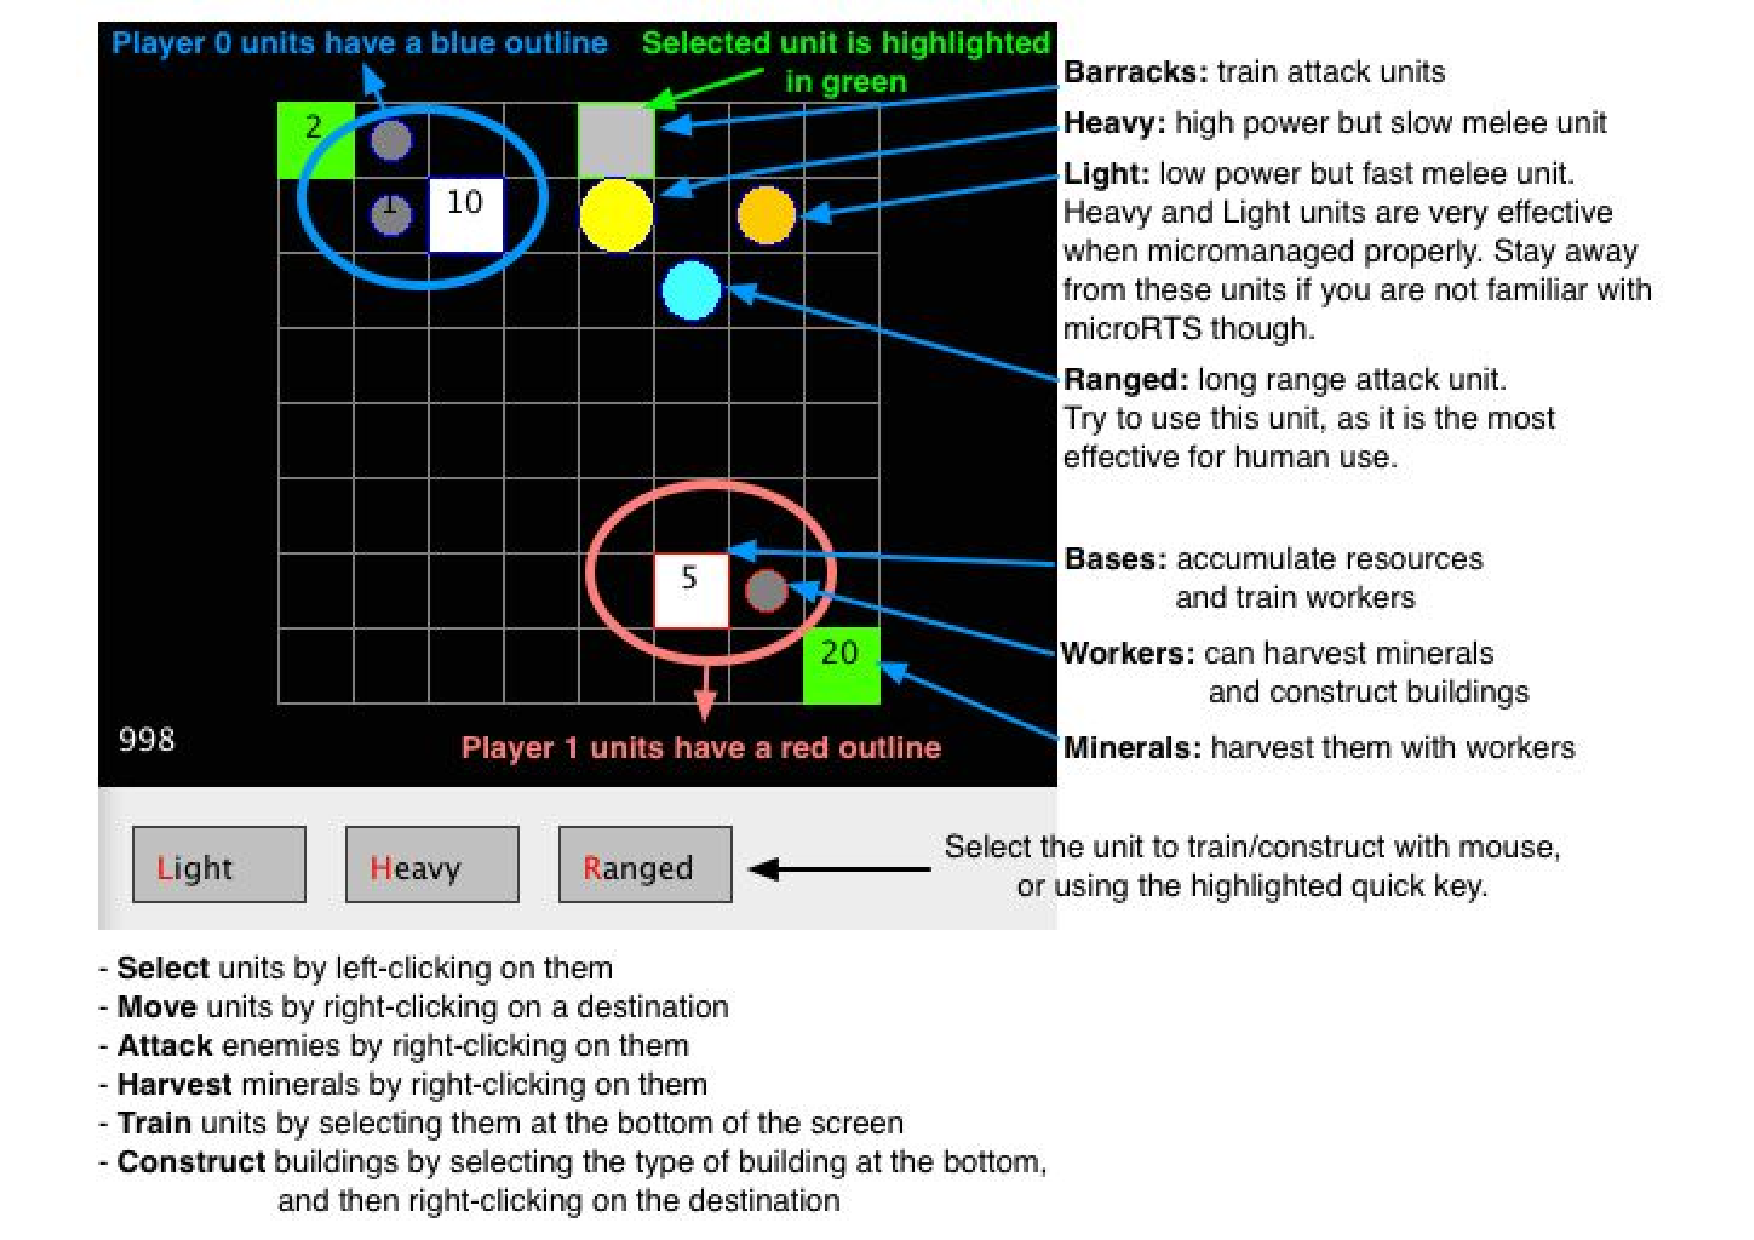
\includegraphics[width=0.8\textwidth]{fig/microrts.pdf}
%%%%	\caption{Uma foto da tela do MicroRTS}
%%%%	\label{fig:microrts}
%%%%\end{figure} \msr{alterar essa imagem pro uma sem legenda?}
%%%%
%%%%No ambiente há algumas estrategias implementadas, cada estrategia possui variações dos algoritmos. Algumas das estrategias são:
%%%%\begin{itemize}
%%%%	\item Minimax Alpha-Beta Search Strategies - O que muda entre as técnicas é o jeito com que é feito a expansão do grafo.
%%%%	\item Monte Carlo Search Strategies - Executa jogadas aleatórias para planejar e após utiliza uma heurística para determinar em qual caminho seguir.
%%%%\end{itemize}
%%%%
%%%%%\frm[inline]{E.. depois da itemização talvez seja interessante concluir algo}
%%%%A plataforma já foi utilizada para aplicar técnica de IA. Por esse motivo a utilização desta plataforma se torna viável. A comparação entre as estrategias já existentes com a que estou propondo pode mostrar que a abordagem resulta em um melhor desempenho. 
